%% Canonical IEEEtran manuscript. Generated tables and figures derive from recorded data.
\documentclass{IEEEtran}
\usepackage{cite}
\usepackage{amsmath,amssymb,amsfonts}
\usepackage{graphicx}
\usepackage{booktabs}
\usepackage{xcolor}
\usepackage{url}
\usepackage{tikz}
\usepackage{placeins}
\usetikzlibrary{arrows.meta,positioning}
% Auto-generated numeric values.
\newcommand{\TrialCount}{14}
\newcommand{\SensorRows}{65,697}
\newcommand{\CaptureMinutes}{23.13}
\newcommand{\ObservedSeconds}{1348.69}
\newcommand{\GapSeconds}{39.20}
\newcommand{\GapCount}{57}
\newcommand{\GapPercent}{2.82}
\newcommand{\StaleRows}{40}
\newcommand{\FailClosedRows}{110}
\newcommand{\DecisionRows}{65,684}
\newcommand{\EventMotionSeconds}{236.31}
\newcommand{\BlockResponses}{31}
\newcommand{\FollowupCodes}{11}
\newcommand{\IntakeCodes}{18}
\newcommand{\CompleteSurveyCodes}{9}
\newcommand{\LegacyErrorLow}{0.413}
\newcommand{\LegacyErrorHigh}{0.534}
\newcommand{\StableBlockMedians}{29}
\newcommand{\EventFreshRows}{13,048}
\newcommand{\EventMotionRowsLow}{11,509}
\newcommand{\EventMotionRowsMain}{11,355}
\newcommand{\EventMotionRowsHigh}{11,319}
\newcommand{\SafetyPreMean}{3.82}
\newcommand{\SafetyPostMean}{4.45}
\newcommand{\SafetyMeanChange}{0.64}
\newcommand{\TrustPreMean}{4.00}
\newcommand{\TrustPostMean}{4.18}
\newcommand{\TrustMeanChange}{0.18}

\begin{document}
\title{Context-Aware Speed and Separation Monitoring for Human--Robot
Ceiling-Panel Installation: An Exploratory Evaluation}
\author{Zenan Wu, Luke Siniakov, and Michael Magila%
\thanks{The authors are with the Department of Civil Engineering, Monash
University, Melbourne, Australia. This work is a 2026 Final Year Project
supervised by Yihai Fang.}%
}
\maketitle
\begin{abstract}
Overhead panel installation requires a worker and a robot to coordinate around
a shared payload, a setting in which fixed protective zones cannot distinguish
approaching, working and retreating behaviour and therefore interrupt the task
more often than necessary. This paper presents a context-aware speed and
separation monitoring (SSM) controller for human--robot ceiling-panel
installation and its evaluation on a physical prototype. A three-state
Gaussian-mixture hidden Markov model (HMM) recognises the task phase from
motion-capture features, a kinematic predictor detects rapid intrusion toward
the robot, and a deterministic command ceiling guarantees that neither learned
output can raise the robot speed above the reactive separation envelope. In
leave-one-operator-out validation the causal phase recogniser reached 0.794
accuracy and 0.725 balanced accuracy. Twelve participants completed a
counterbalanced three-block protocol with fixed, reactive and predictive
controllers; 14 telemetry trials and 31 block questionnaires were analysed.
Participants reported high confidence that the robot would stop and low
workload, and mean perceived safety rose from \SafetyPreMean{}/5 before the
session to \SafetyPostMean{}/5 after it. The telemetry showed that the choice of
geometric reference and the execution of cued movements materially change how
the recorded control behaviour should be read. The study demonstrates the
integration of task-phase recognition, intrusion prediction and multimodal
sensing in a construction-style task, and identifies the measurement
requirements for a conclusive comparison of the three controllers.
\end{abstract}

\begin{IEEEkeywords}
Human--robot collaboration, speed and separation monitoring, hidden Markov model,
construction robotics, motion capture, human factors.
\end{IEEEkeywords}

\section{Introduction and Background}
\IEEEPARstart{O}{verhead} panel installation combines handling, alignment and
fastening in a workspace shared by a worker and a moving payload. A robot can
support the panel while the worker supplies judgement and dexterity. However,
the worker's position changes during the task, the payload enlarges the occupied
volume, and unnecessary stops can disrupt coordination.

Speed and separation monitoring (SSM) depends on protective separation and timely
protective action \cite{iso10218_2_2025,iso15066,marvel2017implementing}. A fixed
threshold is transparent but does not distinguish approaching, stationary and
retreating motion. Task context may improve coordination, provided recognition errors cannot relax
the deterministic command bound. The controller presented here therefore
separates task-phase recognition, kinematic prediction and geometric
constraints.

The research question is whether task context can improve coordination beyond
fixed-zone and reactive policies while remaining bounded by the same geometric
constraint. The intended comparison considers intrusion response, unnecessary
interruption, task efficiency and participant experience. The present exploratory
analysis addresses three supporting questions: how accurately the model recognises
task phase under causal operation; how geometry and cued movement affect the
interpretation of recorded control behaviour; and what the questionnaire responses
show about the experience of successive task blocks. These questions characterise
the prototype and the evidence needed to evaluate the original comparative aim.

The work contributes a physical ceiling-panel collaboration prototype that
separates task-phase recognition from kinematic intrusion prediction under an
explicit command ceiling; a descriptive analysis of geometric inputs and robot
motion during the task; and item-level human-experience results with a
complete-response sensitivity analysis. The contribution is the application-specific integration and evaluation of these
elements rather than a new SSM formulation.

\section{Related Work}
\subsection{Construction HRC}
Robotic construction research has increasingly moved from isolated automation
toward systems in which human expertise and robot strength are combined
\cite{bock2015construction,zhang2023construction}. Reviews of construction HRC
identify safety, perception, communication and task allocation as continuing
barriers to deployment \cite{wei2023construction,lin2025safety}. Panel installation
is an appropriate case study because the person and robot must coordinate around a
shared object and because excessive conservative stopping directly affects task
fluency.

\subsection{Speed and Separation Monitoring}
SSM requires more than a fixed radius around the robot. The required separation
depends on human and robot motion during sensing, controller reaction and robot
stopping, together with intrusion and position-uncertainty allowances
\cite{marvel2017implementing,iso15066}. Byner et al.\ \cite{byner2019dynamic}
derive robot velocity limits using separation and motion direction, and evaluate
cycle performance in a physical machine-tending task. Karagiannis et al.\
\cite{karagiannis2022adaptive} switch safety-zone configurations according to robot
position, using an overhead safety camera, a safety-rated programmable logic
controller (PLC) and the robot controller in an automotive-inspired cell. These studies establish that adaptation and productivity evaluation are
already part of SSM research, and they define the reactive comparator against
which task context must show incremental value.

Construction-specific work further narrows the contribution. Xiao Lin et al.\
\cite{lin2025digitaltwin} integrate worker, robot and material geometry in a digital
twin with dynamic protective-distance calculation, evaluating static and dynamic
conflict scenarios. Their treatment of manipulated materials is particularly
relevant to panel installation, because a proxy around the robot alone does not
describe the occupied volume once a panel is carried. Table~\ref{tab:prior-work}
summarises how these approaches relate to the present prototype.

\subsection{Human Activity Recognition and Collaboration}
Hidden Markov models (HMMs) provide an interpretable probabilistic representation
of temporal state. They describe a hidden state sequence through a transition
matrix and relate each state to observable measurements through an emission model
\cite{rabiner1989}. HMMs have been used in wearable activity recognition and
human--robot task modelling \cite{manouchehri2023hmm,berg2018assembly}. However,
task phase and hazard are different variables: a person can trip while approaching,
working or retreating. This project therefore uses the HMM only for task context. The rapid-intrusion
event is detected separately by the kinematic intrusion predictor of
Section~\ref{sec:context}, which uses only measured distance and closing speed.

Semantic states such as ``working'' or ``retreating'' describe task activity,
whereas a hazardous situation concerns exposure to harm. A rapid approach may
occur within any phase, so treating hazard as a mutually exclusive phase would
confound activity with event recognition. Separating these variables keeps the
geometric command bound testable independently of the HMM's interpretation.

A closely related construction study by Xiao Lin et al.\
\cite{lin2026semantic} combines a semantic workflow model, policies learned from
demonstration and local safety control in a virtual-reality wall-panel task with
simulated sensors. The present study complements that work by evaluating a
physical ceiling-panel prototype with measured robot telemetry and participant
questionnaires.

Objective collaboration fluency is commonly evaluated through temporal measures
such as human idle time, robot idle time, concurrent activity and functional delay
\cite{hoffman2019fluency}. Perceived workload and trust can add explanatory
evidence, but subjective reports cannot establish physical safety or replace
measured response \cite{hart1988tlx,jian2000trust}.

The evaluation in this paper therefore connects task recognition, measured
control inputs and perceived experience in a physical panel task.

\begin{table*}[!t]
\centering
\caption{Selected related methods and their relationship to the present study.}
\label{tab:prior-work}
\footnotesize
\begin{tabular}{@{}p{.19\textwidth}p{.38\textwidth}p{.38\textwidth}@{}}
\toprule
Study & Method and evaluation setting & Implication for this study \\
\midrule
Byner et al.\ \cite{byner2019dynamic} & Continuous velocity limits from separation and motion direction; physical machine-tending cycle evaluation. & Reactive speed adaptation is an established comparator; phase recognition must demonstrate incremental value. \\
Karagiannis et al.\ \cite{karagiannis2022adaptive} & Robot-position-dependent zone switching; overhead safety camera and safety PLC in an automotive-inspired cell. & A software command bound is distinct from a safety architecture implemented with safety components. \\
X. Lin et al.\ \cite{lin2025digitaltwin} & Dynamic protective distance with worker, robot and material geometry; construction conflict scenarios. & Panel and body geometry require validation beyond point-proxy arithmetic consistency. \\
X. Lin et al.\ \cite{lin2026semantic} & Learned semantic workflow and local safety control; VR wall-panel installation with simulated sensors. & Task-aware safety control already exists; physical telemetry and reported experience define the present evaluation focus. \\
Present study & Causal HMM phase context and kinematic prediction beneath a command ceiling; physical ceiling-panel prototype. & Telemetry and questionnaire evaluation of a construction-style task with a human participant in the loop. \\
\bottomrule
\end{tabular}
\end{table*}


\section{System Design}
\label{sec:system}
\begin{figure*}[!t]
\centering
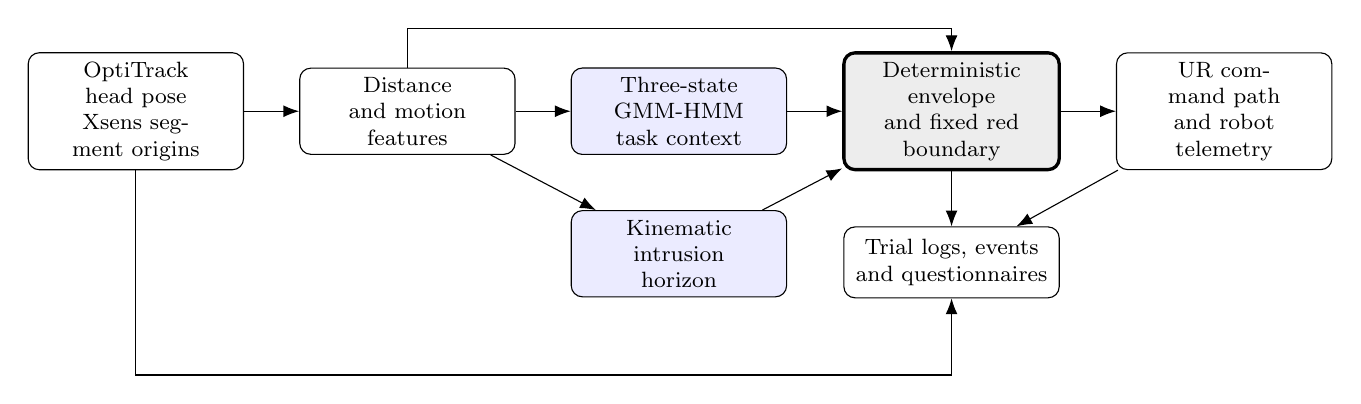
\begin{tikzpicture}[
  node distance=7mm and 7mm,
  box/.style={draw, rounded corners, align=center, minimum height=9mm,
              text width=25mm, font=\footnotesize},
  safety/.style={box, fill=gray!14, very thick},
  learned/.style={box, fill=blue!8},
  every edge/.style={draw, -{Latex[length=2mm]}}
]
\node[box] (sense) {OptiTrack head pose\\Xsens segment origins};
\node[box, right=of sense] (features) {Distance and motion\\features};
\node[learned, right=of features] (context) {Three-state GMM-HMM\\task context};
\node[learned, below=of context] (horizon) {Kinematic intrusion\\horizon};
\node[safety, right=of context] (shield) {Deterministic envelope\\and fixed red boundary};
\node[box, right=of shield] (robot) {UR command path\\and robot telemetry};
\node[box, below=of shield] (log) {Trial logs, events\\and questionnaires};
\path (sense) edge (features)
      (features) edge (context)
      (features) edge (horizon)
      (context) edge (shield)
      (horizon) edge (shield)
      (shield) edge (robot)
      (shield) edge (log)
      (robot) edge (log);
\draw[draw,-{Latex[length=2mm]}] (sense.south) -- ++(0,-26mm) -| (log.south);
\draw[draw,-{Latex[length=2mm]}] (features.north) -- ++(0,5mm) -| (shield.north);
\end{tikzpicture}
\caption{Prototype architecture. Learned outputs (blue) can add caution but cannot raise
the command above the deterministic envelope (grey). Sensing, decisions, commands
and measured robot response are logged for every trial.}
\label{fig:architecture}
\end{figure*}


\subsection{Overview}
The controller (Fig.~\ref{fig:architecture}) takes as input the position and
velocity of the worker relative to the robot, obtained from motion capture, and
the robot's tool position, obtained from the robot controller. Its output is a
single speed fraction in $[0,1]$ that is applied to the robot's speed override,
with a pause request when the fraction is zero. The remainder of this section
describes the apparatus, the geometric features, the task-context and intrusion
models, and the policies that map these to the command.

\subsection{Apparatus and Sensing}
\label{sec:apparatus}
The laboratory prototype (Fig.~\ref{fig:apparatus}) uses a Universal Robots UR10
six-axis arm fitted with a vacuum gripper that carries a lightweight
ceiling-panel surrogate. The arm lifts the panel to ceiling height, the
participant approaches to work on the raised panel, and the arm lowers it again.
The participant's motion is measured by two independent systems.

\emph{Xsens MVN} is a wearable inertial motion-capture suit. Seventeen small
inertial measurement units, each containing an accelerometer, gyroscope and
magnetometer, are strapped to body segments. Their signals are fused with a
biomechanical model into the position and orientation of 23 body segments
(pelvis, spine, head, arms, legs and feet) at up to 240~Hz
\cite{roetenberg2009xsens,schepers2018xsens}. Because position is obtained by
integrating inertial signals, the estimate drifts slowly in the world frame,
and its origin is set by a calibration pose rather than by the room. In this
work the Xsens path supplies the body-segment origins used as the controller's
body-distance input in the later geometry version.

\emph{OptiTrack} is an optical motion-capture system. Several infrared cameras
mounted around the cell (visible on the frame in Fig.~\ref{fig:apparatus}a)
observe passive reflective markers, and the Motive software triangulates each
marker to millimetre-level position in a fixed room coordinate frame
\cite{optitrack2024motive}. A cluster of markers on the participant's head
cap is tracked as a single rigid body. OptiTrack therefore supplies an absolute
head position relative to the robot without drift, but it does not describe the
rest of the body. In this work the OptiTrack head position is the input to the
distance and closing-speed features that drive the phase model and the reactive
envelope.

The two systems are combined by role rather than by fusing their estimates:
OptiTrack provides the absolute head position relative to the robot, and Xsens
provides body posture. Both streams enter the same feature extractor through a
common sample interface, so the controller is independent of which tracker
supplied a sample. Robot telemetry from the UR controller supplies the tool
centre point (TCP) pose, that is the position of the gripper face, and the six
joint velocities. The control loop runs at a nominal 60~Hz and the actual sample
intervals are logged.

\begin{figure*}[!t]
\centering
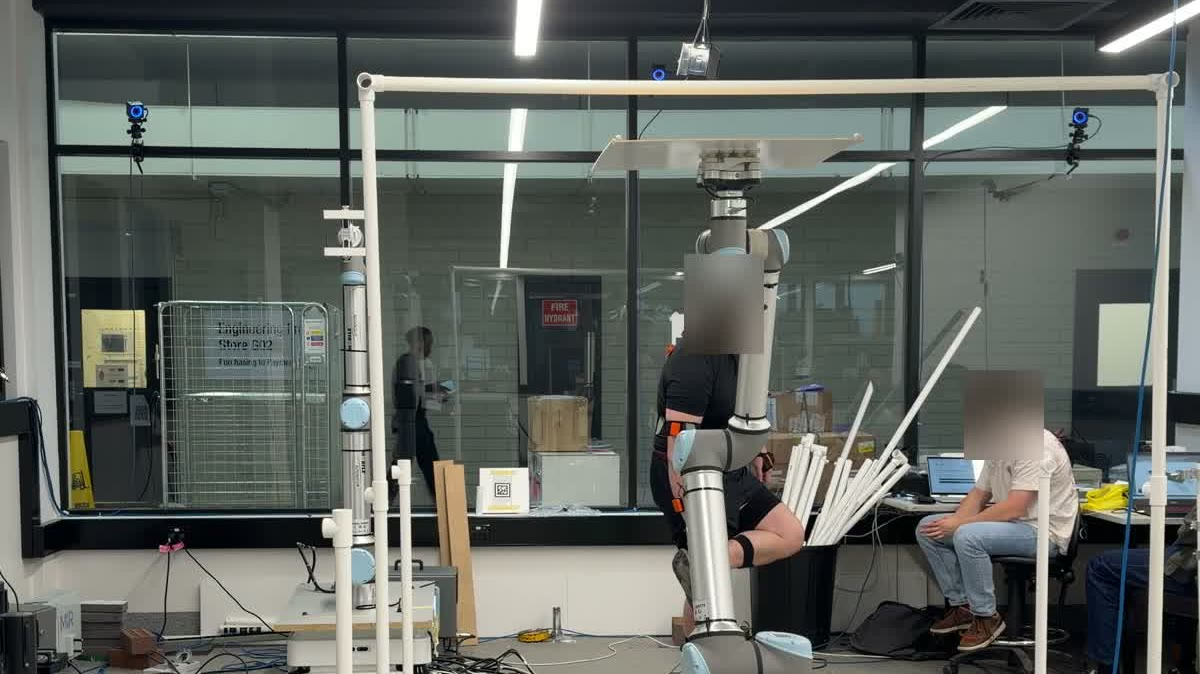
\includegraphics[width=.325\textwidth]{figures/apparatus-a.jpg}\hfill
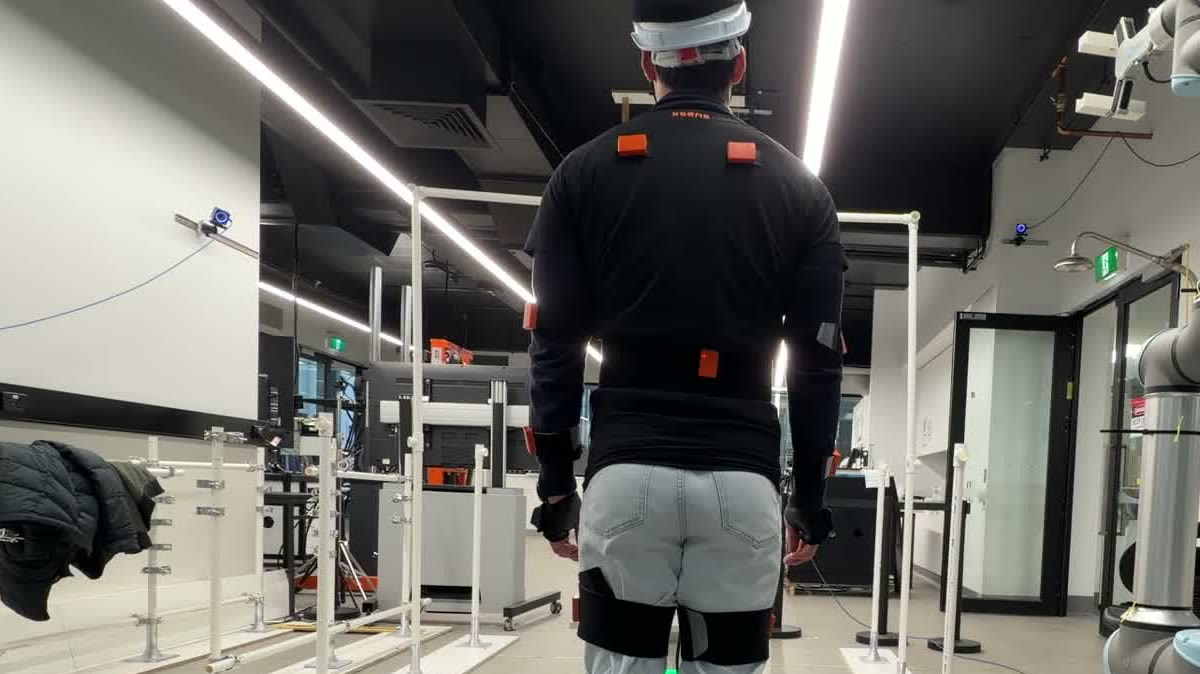
\includegraphics[width=.325\textwidth]{figures/apparatus-b.jpg}\hfill
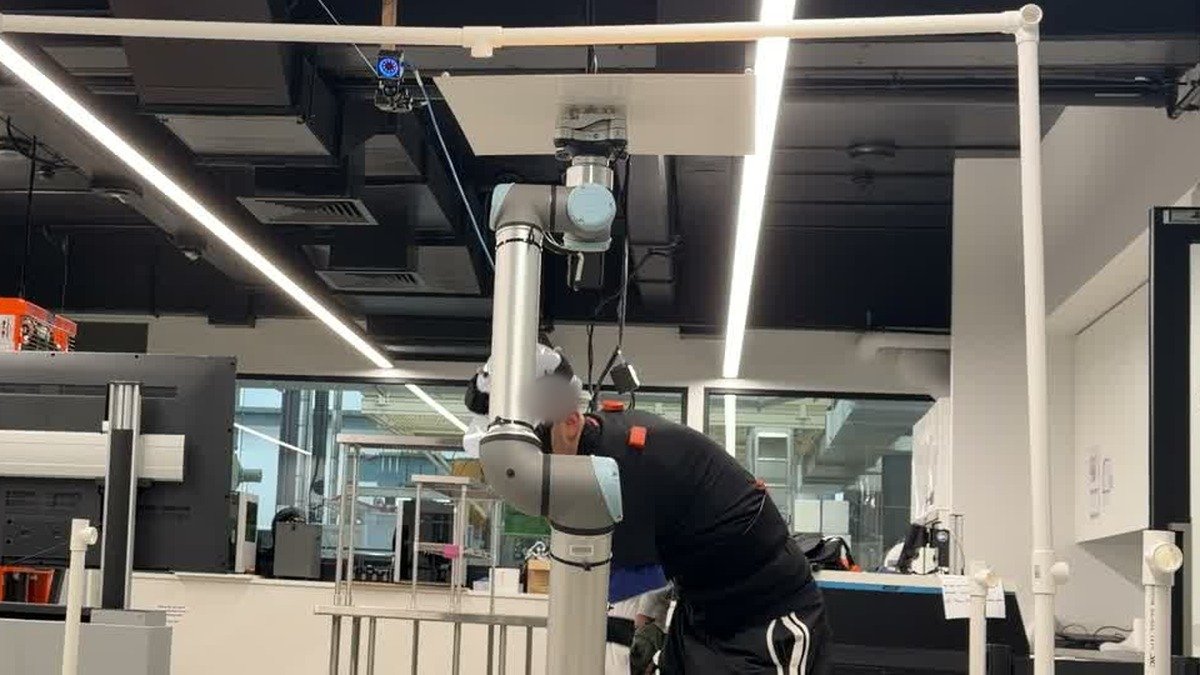
\includegraphics[width=.325\textwidth]{figures/apparatus-c.jpg}
\caption{Laboratory apparatus. (a) The cell: UR10 arm holding the panel surrogate
at ceiling height, OptiTrack cameras on the overhead frame, and the operator
desk. (b) A participant wearing the Xsens MVN suit and OptiTrack head cap,
viewed from behind while approaching the robot. (c) The working phase: the
participant works beneath the raised panel. Faces are obscured.}
\label{fig:apparatus}
\end{figure*}

\subsection{Geometry Versions}
For a tracked point $\mathbf p$ (the head position) and the nearest point
$\mathbf q$ on a vertical column proxy that stands in for the robot, the head
features are
\begin{equation}
d=\|\mathbf q-\mathbf p\|_2,\qquad
v_{\rm proj}=\mathbf v^{\mathsf T}\mathbf u,
\end{equation}
where $d$ is the separation distance in metres, $\mathbf v$ is the head velocity
estimated from the slope of recent samples, $\mathbf u$ is the unit vector from
the head toward the proxy, and $v_{\rm proj}$ is the closing speed in m/s;
positive $v_{\rm proj}$ means the person is moving toward the robot. Heading
alignment $h_t$, used later, is the alignment of the velocity vector with
$\mathbf u$, not torso orientation. Table~\ref{tab:notation} collects the
symbols used in this section.

\begin{table}[!t]
\centering
\caption{Notation used in the controller equations.}
\label{tab:notation}
\footnotesize
\begin{tabular}{@{}lp{5.1cm}@{}}
\toprule
Symbol & Meaning \\
\midrule
$d$ & Separation between tracked point and robot proxy (m) \\
$v_{\rm proj}$, $a_{\rm proj}$ & Closing speed (m/s) and closing acceleration (m/s$^2$) \\
$h_t$ & Velocity-heading alignment with the robot direction \\
$z_t$ & Hidden task phase at time $t$ (approaching, working, retreating) \\
$w_{ik},\boldsymbol\mu_{ik},\boldsymbol\sigma^2_{ik}$ & Weight, mean, variance of mixture component $k$, phase $i$ \\
$r_{\rm red}$ & Radius of the fixed inner (red) boundary (m) \\
$\tau$ & Predicted time to reach the red boundary (s) \\
$S$ & Protective separation distance (m) \\
$T$ & Assumed reaction plus stopping time (s) \\
$C$ & Intrusion allowance for body parts not tracked (m) \\
$S_a$ & Allowance for sensing uncertainty (m) \\
$u_{\rm env},u_{\rm context},u_{\rm cmd}$ & Envelope, context, commanded speed fractions (0--1) \\
\bottomrule
\end{tabular}
\end{table}

Two geometry implementations were used during data collection. (Throughout
this paper a code such as P17 denotes a study ID assigned to one recorded
participant session, and T05 a trial within it; see
Section~\ref{sec:participants}.) Sessions P17 and P22 use head features that are
not arithmetically consistent with a same-row live-TCP column reconstruction. P24 records a live TCP reference for the head feature and
an anchored set of segment origins for the controller's body-distance input.
The phase model uses head-derived features in both versions. The two versions
are reported separately throughout.

\subsection{Task Context and Intrusion Prediction}
\label{sec:context}
The three hidden phases are approaching, working and retreating. The observation
vector is $\mathbf x_t=[d_t,v_{{\rm proj},t},\|\mathbf v_t\|,h_t]^{\mathsf T}$,
where $h_t$ is velocity-heading alignment. Each state's emission density is a
three-component diagonal Gaussian mixture:
\begin{equation}
p(\mathbf x_t\mid z_t=i)=\sum_{k=1}^{3}w_{ik}
\mathcal N(\mathbf x_t;\boldsymbol\mu_{ik},\operatorname{diag}
(\boldsymbol\sigma^2_{ik})),
\end{equation}
where $z_t$ is the hidden phase at time $t$, $w_{ik}$ is the weight of mixture
component $k$ for phase $i$ (the three weights sum to one), and
$\boldsymbol\mu_{ik}$ and $\boldsymbol\sigma^2_{ik}$ are that component's mean
and per-feature variance. The online forward filter uses present and past observations; offline Viterbi
decoding also uses subsequent observations. Their validation values are therefore
reported separately. Long labelled phases and the transition prior produce highly persistent
states, which may delay recognition of short movements.

The intrusion channel operates independently of the HMM. It solves
\begin{equation}
d-r_{\rm red}-v_{\rm proj}\tau-\tfrac12 a_{\rm proj}\tau^2=0
\end{equation}
for the time $\tau$ at which the person, continuing at the current closing speed
$v_{\rm proj}$ and closing acceleration $a_{\rm proj}$, would reach the fixed
inner boundary of radius $r_{\rm red}$ from the current separation $d$. A
non-negative $\tau$ within a 0.5-s horizon triggers the intrusion state. The configured closing-speed gate
is 0.6~m/s and projected acceleration is limited to $\pm4$~m/s$^2$.
The predictor detects approach to the boundary; it does not infer intent.

\subsection{Controller Policies and Command Path}
The fixed controller maps constant distance bands to full speed, reduced speed
and a zero request. The reactive controller uses closing speed in a simplified
envelope. The predictive controller adds phase caution and intrusion prediction
to that envelope. Its separation parameterisation is
\begin{equation}
S=\max(0,v_{\rm proj})T+C+S_a,
\end{equation}
where $S$ is the protective separation distance the controller tries to keep,
$T$ is the assumed reaction plus stopping time so that $v_{\rm proj}T$ is the
distance the person closes before the robot stops, $C$ is a constant
intrusion allowance for parts of the body that the tracked point does not
cover, and $S_a$ is an allowance for sensing uncertainty. This is the form of
the ISO/TS 15066 separation formula with the robot's own travel term omitted
\cite{iso15066}. The configured values are $T=0.4$~s, $C=0.2$~m and
$S_a=0.1$~m. The ramp above $S$ is
0.3~m. The fixed inner radius is 0.94~m; the fixed yellow radius is 1.6 times
that value. These values were selected for the laboratory cell and are not
measured stopping or uncertainty bounds of an installed system.

In SSM mode, the software constraint is
\begin{equation}
u_{\rm cmd}=\min(u_{\rm env},u_{\rm context}),\qquad 0\le u_{\rm cmd}\le1,
\label{eq:bound}
\end{equation}
where $u_{\rm env}$ is the speed fraction allowed by the reactive envelope,
$u_{\rm context}$ is the fraction proposed from phase context and intrusion
prediction, and $u_{\rm cmd}$ is the fraction sent to the robot. The minimum
means the learned context can only lower the command. A fixed inner-boundary override forces a zero request inside $r_{\rm red}$, and
unavailable tracking is handled conservatively by falling back to the most
restrictive state. The command is applied through the UR speed override and the
controller's pause interface. The prototype is a research controller: its
command path is not a safety-rated protective stop, and the bound in
(\ref{eq:bound}) constrains the software request rather than certifying the
installed system (Section~\ref{sec:limitations}).

\section{Model Development and Validation}
The phase classifier was developed before the participant study using 32
accepted labelled trials recorded by the three team members acting as operators
under study IDs P03 (eight trials), P04 (12) and P05 (12), containing 90,487
frames. Class counts are 17,267 approaching, 53,609 working and 19,611
retreating. Validation used leave-one-operator-out cross-validation.
% AUTO-GENERATED by scripts/make_paper_tables.py.
% DO NOT EDIT BY HAND -- edit the analysis and regenerate (make paper).

\begin{table}[t]
\centering
\caption{Leave-one-operator-out phase-recognition validation on the development set. Viterbi decoding uses the full sequence; the causal filter uses present and past observations.}
\label{tab:model-validation}
\begin{tabular}{lr}
\toprule
Measure & Value \\
\midrule
Development participants & 3 \\
Accepted trials & 32 \\
Labelled frames & 90487 \\
Offline Viterbi accuracy & 0.821 \\
Offline balanced accuracy & 0.757 \\
Causal-filter accuracy & 0.794 \\
Causal-filter balanced accuracy & 0.725 \\
Approaching recall & 0.693 \\
Working recall & 0.923 \\
Retreating recall & 0.654 \\
Offline fold P03 accuracy & 0.812  \\
Offline fold P04 accuracy & 0.817  \\
Offline fold P05 accuracy & 0.832  \\
\bottomrule
\end{tabular}
\end{table}

Two measures are reported. Accuracy is the fraction of all frames whose
predicted phase matches the label; because working frames dominate, a model
that favours the working class scores well on it. Balanced accuracy is the mean
of the three per-class recalls, so each phase counts equally regardless of how
many frames it has. Offline accuracy is 0.821 and causal accuracy is 0.794
(Table~\ref{tab:model-validation}). Balanced accuracy is lower, particularly for
the causal filter (0.725), and the working class has the highest offline recall.
The small development pool, temporal correlation within trials and the use of
the same folds during development limit the generalisation of these values.

\FloatBarrier
\section{Experimental Method}
\label{sec:method}
\subsection{Task and Experimental Design}
The protocol specifies three blocks labelled A, B and C, with fixed, reactive and
predictive conditions assigned through six rotated orders. Each block schedules
one clean, one distractor and one rapid-movement trial. The ceiling-panel sequence
includes approach and loading, retreat before lifting, work near the raised panel,
and retreat before lowering and unloading. The scripted cue is placed during the lift and was delivered by the operator,
so cue windows mark the instruction rather than the measured onset of movement.

\subsection{Participants and Analysed Records}
\label{sec:participants}
Twelve participants completed the protocol under Monash University ethics
approval (project 51642). One further session was aborted for technical
reasons and is excluded. Each session was assigned a study ID (P-number); because
some sessions were restarted with a new ID, the IDs label recorded sessions and
do not map one-to-one onto individuals.

A descriptive analysis was used because complete within-person controller
sequences and consistent participant linkage were unavailable. Telemetry entered
the analysis only where a session's sample stream and event journal were both
readable and internally consistent (Section~\ref{sec:telemetry}); at the time of
analysis this criterion was met by 14 trials from three sessions, P17, P22 and
P24, and the remaining sessions contribute questionnaire data only. The analysis
therefore included 14 telemetry trials associated with three study IDs and 31
block questionnaire submissions associated with 11 IDs. Nine IDs had all three
block questionnaires and two lacked the final block response. Matched intake
and end responses were available for all 11 follow-up IDs. Telemetry and
questionnaire outcomes were analysed separately because their coverage differs.
Recorded samples and original form responses were used directly; no missing
values were imputed.

\subsection{Telemetry Processing}
\label{sec:telemetry}
A trial entered the telemetry analysis when its sample stream and event journal
were readable and its sample count matched the trial metadata. Fourteen trials
from the three sessions named above met these criteria. One additional trial record lacked its sample stream and
was excluded. The resulting dataset contains \SensorRows{} samples.

For timestamps $t_i$, time summaries use left-held values only when
$0<t_{i+1}-t_i\le0.25$~s. Longer intervals are reported separately and excluded
from both numerator and denominator. The final sample has no following exposure
interval. Fresh motion telemetry requires an available packet, six finite joint
velocities and a source age between zero and 0.25~s. A maximum absolute joint
velocity exceeding 0.005~rad/s is a diagnostic motion flag; counts at 0.001 and
0.01~rad/s are retained as threshold sensitivity checks.

Head-feature consistency is assessed by recomputing point-to-column distance
from the same row's head position and live TCP; this is an internal
consistency check rather than an external calibration. Cue-window extrema are
the minimum distance and maximum closing speed within a window and need not
occur at the same instant. Zero-command time includes intentional holds and is
therefore reported as such rather than as false interruption.

\subsection{Questionnaire Inclusion and Scoring}
Questionnaire analysis excluded pilot, link-test and qualification submissions.
There were \IntakeCodes{} intake records, \BlockResponses{} block responses and
\FollowupCodes{} end responses after those exclusions. Block counts were A: 11, B: 11 and C: 9, with no duplicate ID/block keys.

The block questionnaire uses five-point ratings. Three semantic differentials
run from anxious to relaxed, agitated to calm, and quiescent to surprised. Four
agreement items concern stopping confidence, constant monitoring, unnecessary
stopping and speed legibility. Three adapted items concern mental demand,
physical demand and frustration. The workload items are adapted from NASA-TLX \cite{hart1988tlx} and the
confidence and monitoring items from Jian et al.\ \cite{jian2000trust}; neither
subset constitutes the full validated instrument, so items are analysed
individually in their original direction and no composite score is formed.

Block results are presented as raw response counts and median [first, third
quartile], using linear quantile interpolation. A sensitivity summary uses only
the nine complete A--C response sets. Within these sets, counts of increases,
ties and decreases between A and C retain the pairing and original item direction;
they describe sequence-related changes without interpreting higher as uniformly
better. Results are grouped by recorded block label rather than controller
because assignment records alone do not establish the controller each
questionnaire refers to. Intake/end comparisons match study IDs and
retain the change from expected to experienced safety and trust. Both forms use
1 = not at all and 5 = completely.

Because neither the independent sample size nor complete controller exposure
can be established, the analysis is descriptive: no significance tests,
confidence intervals or effect estimates are reported, and missing observations
are not assumed to be random.

\section{Results}
\subsection{Telemetry Characteristics}
The telemetry dataset contains five trials under P17, eight under P22 and one
under P24. P17 and P22 also have block and end questionnaires; P24 has an intake
record. Table~\ref{tab:trials} summarises the recorded controller, scheduled event,
capture span and zero-command proportion for each analysed trial.

% Generated from empirical evidence; do not hand-edit.
\begin{table*}[t]
\centering
\caption{Analysed telemetry trials. Span is capture duration, not isolated task time. Zero-request time includes intentional holds; it is not a false-stop rate.}
\label{tab:trials}
\footnotesize
\begin{tabular}{lllrrrr}
\toprule
Code/trial & Controller & Planned event & Rows & Span (s) & Gaps (s) & Zero request (\%) \\
\midrule
P17 T05 & Fixed & Distractor & 5,186 & 103.2 & 2.45 & 30.1 \\
P17 T06 & Fixed & Clean & 4,550 & 91.7 & 2.55 & 30.8 \\
P17 T07 & Reactive & Clean & 5,061 & 101.1 & 2.88 & 41.3 \\
P17 T08 & Reactive & Distractor & 4,815 & 97.0 & 3.06 & 34.2 \\
P17 T09 & Reactive & Rapid Cue & 4,426 & 92.1 & 2.50 & 32.8 \\
P22 T02 & Reactive & Distractor & 5,415 & 108.3 & 2.31 & 34.4 \\
P22 T03 & Reactive & Rapid Cue & 4,668 & 93.6 & 2.28 & 29.0 \\
P22 T05 & Predictive & Rapid Cue & 5,315 & 109.0 & 3.05 & 34.9 \\
P22 T06 & Predictive & Clean & 4,400 & 90.0 & 2.62 & 27.0 \\
P22 T07 & Predictive & Distractor & 4,950 & 101.1 & 2.75 & 25.9 \\
P22 T08 & Fixed & Rapid Cue & 4,745 & 96.0 & 3.13 & 31.4 \\
P22 T09 & Fixed & Distractor & 4,772 & 95.6 & 2.58 & 24.9 \\
P22 T10 & Fixed & Clean & 4,761 & 95.1 & 2.59 & 25.3 \\
P24 T01 & Predictive & Rapid Cue & 2,633 & 114.2 & 4.45 & 39.9 \\
\bottomrule
\end{tabular}
\par\smallskip\begin{minipage}{\linewidth}\footnotesize Intervals over 250 ms are excluded from time integrals. Zero-request percentage uses the remaining positive intervals as its denominator. P17 and P22 use the earlier head geometry; P24 uses anchored segment origins for control.\end{minipage}
\end{table*}


The \TrialCount{} analysed trials contain \SensorRows{} samples and
\CaptureMinutes{} minutes of summed capture spans
(Table~\ref{tab:trials}). \GapCount{} intervals exceed 250~ms, totalling
\GapSeconds{}~s or \GapPercent{}\% of those spans; \ObservedSeconds{}~s remain
for time integrals. In total 40 rows carry a stale-tracking flag. Controller decisions
exist in \DecisionRows{} rows, of which 110 indicate unavailable tracking and
invoke the conservative controller state.

Zone entries and stop onsets (Table~\ref{tab:trials}) follow the task
structure: every trial contains two to seven entries into the red zone, which
correspond to the loading, working and unloading approaches the task requires,
so red-zone entries are not a count of hazardous events. Stop onsets separate
the controllers more clearly. Fixed and reactive trials contain six to nine
protective-stop onsets each, of which three to five last at least 1~s. The
four predictive trials contain 15, 20, 29 and 73 onsets, but only two or three
per trial last at least 1~s; the remainder are stop segments shorter than
0.5~s in which the command alternated rapidly between stop and run. The
predictive policy therefore did not hold the robot stopped for longer, but it
switched the stop request far more often, and P24~T01, the only trial with the
anchored segment-origin geometry, shows the most switching (68 segments under
0.5~s).

Across ten non-clean cue windows, fresh joint telemetry exceeds the diagnostic
motion threshold for \EventMotionSeconds{}~s of observed intervals. The measurements confirm robot motion during labelled event windows.
Among \EventFreshRows{} fresh telemetry rows in these windows, motion counts are
\EventMotionRowsLow{}, \EventMotionRowsMain{} and \EventMotionRowsHigh{} at
0.001, 0.005 and 0.01~rad/s, respectively. The presence of motion is therefore not sensitive to the chosen threshold.

\subsection{Geometric Inputs and Cued Movements}
The P17/P22 trial-level 95th-percentile discrepancies between recorded head
distance and same-row live-TCP recomputation range from \LegacyErrorLow{} to
\LegacyErrorHigh{}~m (Fig.~\ref{fig:geometry}a). P24's corresponding discrepancy
is below $10^{-12}$~m, showing arithmetic agreement for its head reference.
Arithmetic agreement establishes internal consistency of the P24 geometry; its
physical uncertainty was not measured.

\begin{figure*}[!t]
\centering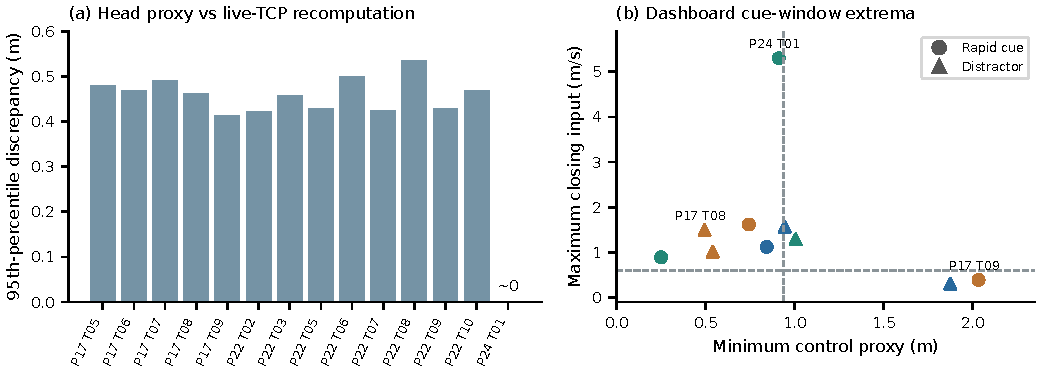
\includegraphics[width=\textwidth]{figures/geometry-and-events.pdf}
\caption{Measurement diagnostics, one mark per trial. (a) For each trial, the
95th-percentile gap between the head distance the controller recorded and the
distance recomputed from the same row's head position and live TCP; P17 and P22
show gaps of 0.4--0.55~m, P24 shows none. (b) For each trial with a cue, the
smallest control-proxy distance reached (horizontal) against the largest closing
speed recorded (vertical) inside the cue window. Dashed lines show the
configured 0.94-m inner boundary and 0.6-m/s closing gate: a rapid cue should
land left of the vertical line and above the horizontal one. Colours identify
fixed (blue), reactive (orange) and predictive (green) records. Geometry
versions differ and the two extrema need not occur at the same instant.}
\label{fig:geometry}
\end{figure*}

Recorded cue labels also differ from their intended kinematics. P17 T09 is labelled
rapid intrusion, yet its minimum controller proxy is 2.034~m and maximum closing
input is 0.388~m/s, below the configured gate. Conversely, the P17 T08 distractor
window reaches a 0.496-m proxy and a 1.494-m/s maximum closing input. P22 T05
reaches a 0.252-m proxy during a rapid cue. These values are controller inputs
rather than validated clearances, and they show that the cue label alone does not
determine the kinematics that were actually recorded.

Figure~\ref{fig:trace} presents the recorded time series for P24 T01. Its rapid-cue
window reaches a 0.913-m controller proxy and a 5.302-m/s maximum closing input.
Command and joint-speed traces are presented together; because the cue marks
the instruction rather than the movement onset, the delay between them is not
reported as a protective response time.

\begin{figure*}[!t]
\centering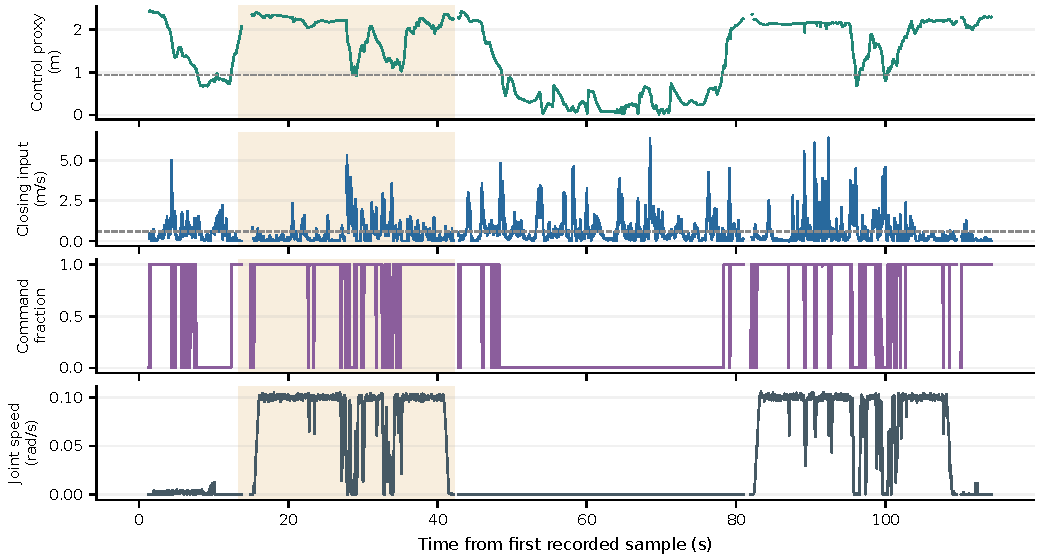
\includegraphics[width=.94\textwidth]{figures/p24-recorded-trace.pdf}
\caption{P24 T01: recorded body-proxy distance, closing input, command fraction
and maximum absolute fresh joint velocity. Shading marks the cue event
window. Dashed lines are configuration thresholds. Gaps over 250~ms break the
lines.}
\label{fig:trace}
\end{figure*}

\subsection{Reported Experience}
Block responses lean toward relaxed/calm, confidence in stopping, and low demand
and frustration (Table~\ref{tab:survey}). Median
stopping confidence is five in each block, while median unnecessary-stopping
agreement is three in A and two in B/C. The latter is a perception item rather than an objective false-stop count,
and responses are clustered within study IDs.

Restricting the analysis to nine complete response sets preserves
\StableBlockMedians{} of the 30 block-item medians. The exception is constant
monitoring in B, whose median changes from two to one. The paired A--C counts
nevertheless reveal variation hidden by marginal medians
(Table~\ref{tab:survey-sensitivity}). Five relaxed ratings increase and four
remain unchanged; none decrease. Unnecessary-stopping ratings increase twice,
decrease twice and remain unchanged five times, despite the lower C median.
Surprise decreases for three codes, increases for two and is unchanged for four.
Thus lower block medians do not establish a common within-code improvement.
% Generated from empirical evidence; do not hand-edit.
\begin{table*}[t]
\centering
\caption{Block questionnaire items: median [first, third quartile]. A, B and C are reported block labels, not pooled controller conditions. All ratings use 1--5.}
\label{tab:survey}
\footnotesize
\begin{tabular}{lrrr}
\toprule
Item & A ($n=11$) & B ($n=11$) & C ($n=9$) \\
\midrule
Anxious to relaxed & 4 [3.5, 4.5] & 5 [4.0, 5.0] & 5 [4.0, 5.0] \\
Agitated to calm & 4 [4.0, 5.0] & 5 [4.0, 5.0] & 5 [4.0, 5.0] \\
Quiescent to surprised & 3 [1.0, 3.0] & 3 [1.0, 4.0] & 1 [1.0, 3.0] \\
Confident robot would stop & 5 [4.0, 5.0] & 5 [4.0, 5.0] & 5 [4.0, 5.0] \\
Had to watch constantly & 2 [1.0, 3.0] & 2 [1.0, 3.0] & 1 [1.0, 3.0] \\
Stopped more than needed & 3 [2.0, 4.0] & 2 [1.0, 3.5] & 2 [2.0, 3.0] \\
Speed changes made sense & 5 [3.5, 5.0] & 5 [4.0, 5.0] & 4 [4.0, 5.0] \\
Mental demand & 1 [1.0, 3.0] & 1 [1.0, 2.0] & 1 [1.0, 2.0] \\
Physical demand & 1 [1.0, 3.0] & 1 [1.0, 2.5] & 1 [1.0, 3.0] \\
Frustration & 1 [1.0, 3.0] & 1 [1.0, 2.0] & 1 [1.0, 1.0] \\
\bottomrule
\end{tabular}
\par\smallskip\begin{minipage}{\linewidth}\footnotesize Higher means the right-hand semantic anchor for the first three items, stronger agreement for the next four, and greater demand/frustration for the final three. Responses are clustered within 11 study IDs; individual-level linkage is incomplete. No trust, safety or workload composite is used.\end{minipage}
\end{table*}

% Generated from empirical evidence; do not hand-edit.
\begin{table}[t]
\centering
\caption{Complete response sets: block medians and within-code changes ($n=9$ codes).}
\label{tab:survey-sensitivity}
\footnotesize
\begin{tabular}{@{}lcc@{}}
\toprule
Item & A/B/C & A to C: up/same/down \\
\midrule
Anxious to relaxed & 4/5/5 & 5/4/0 \\
Agitated to calm & 4/5/5 & 3/6/0 \\
Quiescent to surprised & 3/3/1 & 2/4/3 \\
Confident robot would stop & 5/5/5 & 3/4/2 \\
Had to watch constantly & 2/1/1 & 1/5/3 \\
Stopped more than needed & 3/2/2 & 2/5/2 \\
Speed changes made sense & 5/5/4 & 1/5/3 \\
Mental demand & 1/1/1 & 2/6/1 \\
Physical demand & 1/1/1 & 1/6/2 \\
Frustration & 1/1/1 & 1/5/3 \\
\bottomrule
\end{tabular}
\par\smallskip\begin{minipage}{\linewidth}\footnotesize Counts refer to the raw rating direction, not uniformly to improvement. A--C changes describe block sequence, not a controller effect. The same nine codes supply every row.\end{minipage}
\end{table}


Across 11 matched records, mean safety ratings were \SafetyPreMean{}/5 before
and \SafetyPostMean{}/5 after the session. Eight ratings increased, one was
unchanged and two decreased. Mean trust ratings were \TrustPreMean{} before and
\TrustPostMean{} after; five increased, three were unchanged and three decreased
(Table~\ref{tab:global}). The expected-to-experienced wording and incomplete
individual linkage limit interpretation of these differences.
% Generated from empirical evidence; do not hand-edit.
\begin{table}[t]
\centering
\caption{Paired global ratings for 11 codes with intake and end responses. Five-point items; descriptive code-level changes only.}
\label{tab:global}
\footnotesize
\begin{tabular}{lrrrr}
\toprule
Item & Before & After & $\Delta$ & Up/same/down \\
\midrule
Felt safe & 3.82 & 4.45 & 0.64 & 8/1/2 \\
Trust in distance & 4.00 & 4.18 & 0.18 & 5/3/3 \\
\bottomrule
\end{tabular}
\par\smallskip\begin{minipage}{\linewidth}\footnotesize Before/after wording changes from expected to experienced safety/trust. Means summarize coded responses; neither causation nor an interval-scale measurement model is assumed.\end{minipage}
\end{table}


In end responses, C is selected as safest seven times, compared with two each
for A and B. Full-shift choices are C: six, B: three and A: two. Least-safe choices
are distributed across all labels (A: three; B: four; C: four). Since label-to-controller exposure is not fully established, C is not
interpreted as the predictive controller. Four end responses report noticing
changes between blocks and seven do not; the four comments refer to stopping or
slowing sensitivity and to ascent speed. Median reported suit restriction is two
(interquartile range 1.5--3), and no risk or discomfort comments were entered in
the 11 end forms.

\section{Discussion}
\subsection{Context-Aware Control in the Panel Task}
The prototype integrates task context and kinematic prediction while preserving
a deterministic software ceiling on the commanded speed. This architecture
separates two questions: whether a movement belongs to a normal task phase, and
whether the measured trajectory approaches the configured boundary. An HMM
misclassification need not authorise a higher speed than the geometric envelope,
although errors in geometry or timing still affect that envelope.

The development results indicate that phase recognition is strongest during the
longer working phase. The lower causal balanced accuracy compared with overall
accuracy shows why phase accuracy alone is an insufficient measure of practical
benefit. The stop-onset counts make the cost concrete: the predictive policy
produced two to nine times as many protective-stop onsets as the fixed and
reactive policies in the same task, almost all of them sub-0.5-s segments in
which phase caution and the intrusion predictor toggled the request near a
threshold. This chattering is a controller-design defect rather than a
property of the task, and it is largest under the segment-origin geometry,
whose body-distance input is noisier than the head point. Hysteresis or a
minimum stop dwell on the learned inputs would remove it without touching the
deterministic envelope. The reactive reference is therefore an important
comparator when assessing the added value of learned context.

Equation~\ref{eq:bound} also constrains the expected benefit. For identical SSM
inputs, parameters and zone state, the predictive policy cannot request a higher
speed than the reactive policy: prediction and phase caution can only preserve
or reduce the request. Its incremental value would therefore need to arise from
the timing of intervention or changes in subsequent human--robot coordination,
rather than a more permissive instantaneous speed bound. Such a closed-loop
benefit cannot be inferred from phase accuracy or from applying alternative
policies to the same recorded trajectory.

\subsection{Objective Behaviour and Perceived Experience}
The telemetry illustrates changes in the distance input, speed request and
measured joint motion throughout the panel sequence. The difference between
geometric reference configurations materially affects how these signals can be
interpreted. Similarly, variation between scheduled rapid movements and recorded
closing inputs shows that event labels cannot substitute for measured exposure.
These findings are consistent with the need to validate the sensing-to-stopping
chain when implementing SSM \cite{marvel2017implementing}.

Questionnaire responses generally indicate confidence in the robot stopping,
low mental and physical demand, and limited frustration. Mean experienced safety
exceeds mean expected safety in the matched records, whereas the trust difference
is smaller. These observations suggest a positive reported experience of the
laboratory task. However, novelty, supervised operation, repeated exposure and
expectations could all contribute to the pattern. The change cannot be attributed
specifically to the predictive controller.

The complete-response analysis makes the broad descriptive pattern less dependent
on the two missing final-block forms, but does not remove bias from missingness or
resolve individual linkage. Ceiling ratings for stopping confidence and floor
ratings for demand/frustration also leave limited room to distinguish conditions.
The paired stopping and surprise responses show why aggregate medians should be
read alongside within-code changes. Increased familiarity is a plausible
explanation for greater relaxation across blocks, but was not isolated by this
analysis.

The end-of-session preference for block C does not provide a controller ranking:
block labels rotate across controller assignments, and complete exposure linkage
is unavailable. Likewise, subjective agreement that the robot stopped more than
needed is informative about perceived interruption but is not an objective
false-stop rate. Subjective and physical measures address different aspects of
collaboration and should be interpreted together.

\subsection{Safety and Efficiency Interpretation}
Dynamic SSM research motivates evaluation of availability and cycle performance
\cite{byner2019dynamic,karagiannis2022adaptive}. The present study demonstrates
the implementation needed to investigate those outcomes but does not establish
a safety or efficiency advantage. Zero-command time combines intentional holds
and responses to proximity; capture span includes operator actions and cannot
be equated with isolated task time. These quantities therefore do not establish
false interruption, task efficiency or collaboration fluency
\cite{hoffman2019fluency}.

A non-inferiority conclusion would additionally require a justified margin,
validated protective geometry and end-to-end response measurements, none of
which the current analysis provides; absence of a demonstrated difference is
not evidence of equivalent safety.

\subsection{Coverage of the Planned Measures}
The study design specified four system measures (human--robot distance, number
of speed reductions and stops, number of yellow/red zone entries and task
completion time) and four experience measures (safety, comfort, predictability
and trust) for comparison between static and adaptive safety. Distance, zone entries and stop onsets are reported per trial
(Table~\ref{tab:trials}, Figs.~\ref{fig:geometry} and \ref{fig:trace}), with
the caveat that red-zone entries and a share of the stop time arise from the
loading and unloading approaches the task requires, so they are not counts of
unnecessary interruption. Capture span is reported in place of task completion
time because operator actions fall within the span. Safety and trust are reported as intake/end ratings, comfort through the
relaxed and calm items, and predictability through the speed-legibility item.
The static-versus-adaptive comparison remains open for the linkage and
exposure reasons set out below.

\subsection{Limitations}
\label{sec:limitations}
The sample is small and drawn by convenience. Session restarts prevented
reliable linkage of every study ID to a distinct individual, so record counts
cannot be treated as independent participant counts. Two questionnaire sets lack block C, and objective and
subjective records cover different subsets of the study. Missingness may relate
to technical problems or task execution, limiting complete-case interpretation
and generalisation.

The geometric configuration changed during collection. Head points and segment
origins do not represent complete body, tool and payload surfaces, and their
agreement with a geometric calculation does not establish physical calibration.
The controller is a research prototype: the separation envelope is simplified,
the command path uses the ordinary robot speed override rather than a
safety-rated stop, and no end-to-end protective response was measured, so the
results do not support a certified safety claim for the installed system. Cued movements,
operator pacing, visible motion, learning and fatigue may influence both
behaviour and subjective reports. The model-development results are based on
three operators and do not establish generalisation to construction workers.

\subsection{Implications for Further Development}
Future controlled evaluation should maintain a consistent geometry and validate
its uncertainty against the complete moving volume. Synchronized measurements
of physical movement, controller output and robot deceleration would allow
response-time estimation independently of operator cues. Task-phase estimates
could then be evaluated for their incremental benefit over the reactive policy
using verified within-person controller exposure. A persistent study identifier
across restarted sessions would support that comparison without changing the
participant-facing task.

\section{Conclusion}
This paper presented a context-aware speed and separation monitoring
controller for human--robot ceiling-panel installation and evaluated it on a
physical prototype with human participants. The controller combines measured
closing kinematics, three-state task-phase recognition and kinematic intrusion
prediction beneath a deterministic command ceiling, so that learned context can
only make the robot more cautious. Causal phase recognition reached 0.794
accuracy in leave-one-operator-out validation. Across 14 telemetry trials and
31 block questionnaires, participants reported high confidence in the robot
stopping and low workload, and perceived safety rose over the session; the
telemetry showed that geometric reference selection and cue execution govern
how recorded control behaviour should be interpreted. Complete-response
analysis preserved \StableBlockMedians{} of 30 block medians, while paired
changes showed that lower median interruption ratings were not uniform within
participants. Establishing a controller-specific safety or efficiency
advantage requires the consistent geometry, synchronised response
measurement and persistent participant linkage identified here, and these
define the next stage of the work.

\section*{Data Availability}
Analysis scripts, derived tables and figure-generation code accompany the
manuscript. Participant-level data require controlled access. All reported
experimental summaries are calculated from recorded observations without
imputation or substitution of simulated values.

\section*{Acknowledgment}
The authors thank Associate Professor Yihai Fang for his primary supervision
and academic guidance, Yizhe (Will) Wang for day-to-day technical and laboratory
support, and the Construction Robotics Laboratory for providing facilities.

\section*{AI Assistance Declaration}
AI tools assisted with data-processing code, descriptive analysis, figure
production and manuscript drafting and revision.

\bibliographystyle{IEEEtran}
\bibliography{refs}
\end{document}
